\section{AVHRR infrared channel SRFs}
%====================================
\subsection{Gross SRF comparison}
%--------------------------------
Plots of the SRF data for AVHRR channels 3B, 4, and 5 for the NOAA-16 to MetOp-A platforms are shown in appendix \ref{app:srf}. SRF plots for NOAA-16 are shown in figure \ref{fig:avhrr3_n16}, NOAA-17 in figure \ref{fig:avhrr3_n17}, NOAA-18 in figure \ref{fig:avhrr3_n18}, and MetOp-A in figure \ref{fig:avhrr3_metop-a} respectively.

In general, at the scales shown, the SRFs shown in appendix \ref{app:srf} agree quite well. It is at higher magnifications of the SRF data that differences become visible.


\subsection{Interpolation differences}
%-------------------------------------
The main source of differences between the SRFs is due to interpolation. For the AVHRR instruments, the channels responses are typically reported as a function of wavelength (\micron). For the CRTM transmittance production process, we require the SRFs to be,
\begin{itemize}
  \item A function of frequency (\invcm).
  \item At a fixed frequency interval. For broadband infrared instruments, the frequency interval used is 0.1\invcm.
  \item Begun on a 0.1\invcm{} boundary such as 840.0, 900.6, etc.
\end{itemize}
As such, interpolation of the original data is required.

Our regular processing takes the original channel responses and interpolates the data using the IDL\footnote{Interactive Data Language; a scripting language that provides various functionalities for data processing and visualisation} \texttt{SPLINE} function with a tension value of 5.0, selected qualitatively. From the online IDL help\footnote{\href{http://www.ittvis.com/portals/0/pdfs/idl/refguide.pdf}{IDL Reference Guide}; for IDL Version 7.0, November 2007 Edition, see pp2346-2347; Note the download file is quite large.}:

\begin{quote}
If [the tension value] is close to 0, (e.g., .01), then effectively there is a cubic spline fit. If [the tension value] is large, (e.g., greater than 10), then the fit will be like a polynomial interpolation.
\end{quote}

The impacts of the interpolation scheme are shown visually in figures \ref{fig:avhrr3_n16.ch3.srf.zoom} and \ref{fig:avhrr3_n16.ch5.srf.zoom} for NOAA-16 AVHRR/3 channels 3 and 5; figures \ref{fig:avhrr3_n17.ch4.srf.zoom} and \ref{fig:avhrr3_n17.ch5.srf.zoom} for NOAA-17 AVHRR/3 channels 4 and 5; figures \ref{fig:avhrr3_n18.ch3.srf.zoom} and \ref{fig:avhrr3_n18.ch4.srf.zoom} for NOAA-18 AVHRR/3 channels 3 and 4; and in figures \ref{fig:avhrr3_metop-a.ch3.srf.zoom} and \ref{fig:avhrr3_metop-a.ch5.srf.zoom} for MetOp-A AVHRR/3 channels 3 and 5. Only two channels from each instrument are shown with the understanding that the third channel exhinbits the same sort of differences.

For both the NOAA-16 and NOAA-17 instruments, the current SRF data was linearly interpolated from a much lower resolution dataset, and subsequent spline interpolations have little effect. The impact of the spline interpolation on the lower resolution official SRF data is clearly evident. Note also that there is a slight vertical extent difference between the current and official SRF data -- this is most likely due to renormalisation of the SRFs.

In the NOAA-18 AVHRR/3 case, the SRF datasets coincide almost exactly. The differences that do remain can be attributed to the number of decimal places to which the original and intermediate data was reported in ASCII datafiles.

The current SRF data used for MetOp-A AVHRR/3 clearly suffers from quantisation of the data in the original ASCII datafile (reported to only three decimal places). This data was supplied directly by ITT \citep{Sullivan_avhrr3_metop-a_srf} and, at the time, was the only data available. The offical SRF data from \citet{NESDIS_AVHRR_SRFs} is listed as being modified on 04/21/2008, but it is not yet known if those modifications addressed the quantisation problem.

\begin{figure}[htp]
  \centering
  \includegraphics[scale=1]{graphics/zoom/avhrr3_n16.ch3.srf.zoom.eps}
  \caption{Zoom of NOAA-16 AVHRR/3 channel 3B SRF comparison. \textbf{(a)} Complete SRFs showing zoom region 1. \textbf{(b)} Magnification of SRF section from (a) showing zoom region 2.  \textbf{(c)} Magnification of SRF section from (b).}
  \label{fig:avhrr3_n16.ch3.srf.zoom}
\end{figure}

\begin{figure}[htp]
  \centering
  \includegraphics[scale=1]{graphics/zoom/avhrr3_n16.ch5.srf.zoom.eps}
  \caption{Zoom of NOAA-16 AVHRR/3 channel 5 SRF comparison. \textbf{(a)} Complete SRFs showing zoom region 1. \textbf{(b)} Magnification of SRF section from (a) showing zoom region 2.  \textbf{(c)} Magnification of SRF section from (b).}
  \label{fig:avhrr3_n16.ch5.srf.zoom}
\end{figure}

\begin{figure}[htp]
  \centering
  \includegraphics[scale=1]{graphics/zoom/avhrr3_n17.ch4.srf.zoom.eps}
  \caption{Zoom of NOAA-17 AVHRR/3 channel 4 SRF comparison. \textbf{(a)} Complete SRFs showing zoom region 1. \textbf{(b)} Magnification of SRF section from (a) showing zoom region 2.  \textbf{(c)} Magnification of SRF section from (b).}
  \label{fig:avhrr3_n17.ch4.srf.zoom}
\end{figure}

\begin{figure}[htp]
  \centering
  \includegraphics[scale=1]{graphics/zoom/avhrr3_n17.ch5.srf.zoom.eps}
  \caption{Zoom of NOAA-17 AVHRR/3 channel 5 SRF comparison. \textbf{(a)} Complete SRFs showing zoom region 1. \textbf{(b)} Magnification of SRF section from (a) showing zoom region 2.  \textbf{(c)} Magnification of SRF section from (b).}
  \label{fig:avhrr3_n17.ch5.srf.zoom}
\end{figure}

\begin{figure}[htp]
  \centering
  \includegraphics[scale=1]{graphics/zoom/avhrr3_n18.ch3.srf.zoom.eps}
  \caption{Zoom of NOAA-18 AVHRR/3 channel 3B SRF comparison. \textbf{(a)} Complete SRFs showing zoom region 1. \textbf{(b)} Magnification of SRF section from (a) showing zoom region 2.  \textbf{(c)} Magnification of SRF section from (b).}
  \label{fig:avhrr3_n18.ch3.srf.zoom}
\end{figure}

\begin{figure}[htp]
  \centering
  \includegraphics[scale=1]{graphics/zoom/avhrr3_n18.ch4.srf.zoom.eps}
  \caption{Zoom of NOAA-18 AVHRR/3 channel 4 SRF comparison. \textbf{(a)} Complete SRFs showing zoom region 1. \textbf{(b)} Magnification of SRF section from (a) showing zoom region 2.  \textbf{(c)} Magnification of SRF section from (b).}
  \label{fig:avhrr3_n18.ch4.srf.zoom}
\end{figure}


\begin{figure}[htp]
  \centering
  \includegraphics[scale=1]{graphics/zoom/avhrr3_metop-a.ch3.srf.zoom.eps}
  \caption{Zoom of MetOp-A AVHRR/3 channel 3B SRF comparison. \textbf{(a)} Complete SRFs showing zoom region 1. \textbf{(b)} Magnification of SRF section from (a) showing zoom region 2.  \textbf{(c)} Magnification of SRF section from (b).}
  \label{fig:avhrr3_metop-a.ch3.srf.zoom}
\end{figure}

\begin{figure}[htp]
  \centering
  \includegraphics[scale=1]{graphics/zoom/avhrr3_metop-a.ch5.srf.zoom.eps}
  \caption{Zoom of MetOp-A AVHRR/3 channel 5 SRF comparison. \textbf{(a)} Complete SRFs showing zoom region 1. \textbf{(b)} Magnification of SRF section from (a) showing zoom region 2.  \textbf{(c)} Magnification of SRF section from (b).}
  \label{fig:avhrr3_metop-a.ch5.srf.zoom}
\end{figure}

